\documentclass[10pt]{article}

\usepackage{amsmath}
%
\usepackage{amssymb}
%
\usepackage{enumerate}
%
\usepackage[width=7in,height=10in,top=0.75in,centering]{geometry}
%
\usepackage[dvipsnames]{xcolor}
%
\usepackage{tikz}
%
\usepackage{multicol}
%
\usepackage{hyperref}
%
\usepackage{marginnote}
%
%%%%%%%%%%%%%%%% HEADER %%%%%%%%%%%%%%%%%%%%%
\usepackage{fancyhdr}
\pagestyle{fancy}
%%
%\lfoot{Left footer}
%\cfoot{Center of footer}
%\rfoot{Right of footer}
%%
\lhead{Survey of Calculus I}
\chead{Week 2 Workshop}
\rhead{\thepage}
%
%%%%%%%%%%%%%%%% HEADER %%%%%%%%%%%%%%%%%%%%%
%
%%%%%%%%%%%%%%%% PGFPLOTS %%%%%%%%%%%%%%%%%%%
\usepackage{pgfplots}
%
\pgfplotsset{every axis/.append style={
                    axis x line=middle,    % put the x axis in the middle
                    axis y line=middle,    % put the y axis in the middle
                    axis line style={<->,color=black}, % arrows on the axis
                    %xlabel={$x$},          % default put x on x-axis
                    ylabel={$y$},          % default put y on y-axis
            }}
%
 \pgfplotsset{compat=1.14}
%
 \usepgfplotslibrary{fillbetween}
%%%%%%%%%%%%%%%% PGFPLOTS %%%%%%%%%%%%%%%%%%%
%
\parindent0pt
\fboxsep=0.25cm
%
\newcommand{\Heading}[2]{\fbox{{\Large\textbf{#1}}}\hfill\fbox{\textbf{#2}}\par\vspace{0.1in}}
%
\newcommand{\Name}[1]{\textbf{Name}:\quad#1\hrulefill}
%
\newcommand{\Target}[1]{\textbf{Learning Target(s):}\quad\fbox{#1}\par\medskip}
%
\DeclareMathOperator{\arcsec}{arcsec}
\DeclareMathOperator{\arccot}{arccot}
\DeclareMathOperator{\arccsc}{arccsc}
%
\newcounter{example}[section]
\newcounter{exercise}[section]
%
\newcommand{\important}[2]{\begin{center}\fbox{\begin{minipage}{.97\textwidth}\noindent\textbf{#1}\par#2\end{minipage}}\end{center}}
%
\newcommand{\defn}[1]{\begin{center}\fbox{\begin{minipage}{.97\textwidth}\reversemarginpar\marginnote{\textbf{Definition}}#1\end{minipage}}\end{center}}
%
\newcommand{\example}[1]{\vspace{0.1in}{\textcolor{blue}{\textbf{Example \stepcounter{example}\theexample.}}}\hspace{0.1in}\reversemarginpar\marginnote{\fbox{\bf #1}}}
%
\newcommand{\exercise}[1]{\vspace{0.1in}{\textcolor{blue}{\textbf{Exercise \stepcounter{exercise}\Alph{exercise}.}}}\hspace{0.1in}\reversemarginpar\marginnote{\fbox{\bf #1}}}

%%%%%%%%%%%% BEGIN DOCUMENT %%%%%%%%%%%%%%%
%%%%%%%%%%%% BEGIN DOCUMENT %%%%%%%%%%%%%%%
%%%%%%%%%%%% BEGIN DOCUMENT %%%%%%%%%%%%%%%
%%%%%%%%%%%% BEGIN DOCUMENT %%%%%%%%%%%%%%%
%%%%%%%%%%%% BEGIN DOCUMENT %%%%%%%%%%%%%%%

\begin{document}

\thispagestyle{empty}

\Heading{MATH 1190 \& 1210 Survey of Calculus I}{\begin{minipage}{0.25\textwidth}\begin{center} Week 1 Workshop:\\ Net Change, AROC, Slope, \& Lines \end{center}\end{minipage}}

\vspace{0.1in}

\Name{} \quad \Target{{\bf\color{ProcessBlue}F1}}

\hrulefill\\

\section{Exercise A Extra Practice}

\begin{enumerate}

\item[(a)] Consider the typical Black Friday sale for televisions and suppose that we wished to model the relationship between sale-hungry \textbf{buyers}, $B$ and the availability of cheaply made \textbf{televisions}, $T$. Assume that these things are related and suppose that we have collected two data points $(B_1, T_1) = (10, 1000)$ and $(B_2, T_2) = (100, 100).$
    \begin{enumerate}
        \item[(i)] What is the net change in available televisions from when the buyer population changed from $10$ to $100$ buyers?
        \item[(ii)]What is the average rate of change of the number of available televisions with respect to the number of buyers?
        \item[(iii)]Assuming the buyer-television model is linear, what is the slope of the graph describing the relationship between number of buyers and number of available televisions?
    \end{enumerate}
\item[(b)] The equation $N = \frac{10}{9}T + 5$ describes the relationship between the temperature $T$ (in Celsius) and the number of ice cream cones purchased from a supermarket in Charlottesville $N$ (in cones).
    \begin{enumerate}
        \item[(i)] What is the slope of the graph that describes the relationship between temperature $T$ and number of ice cream comes sold $N?$
        \item[(ii)]What is the (average) rate of change of the number of ice cream comes sold with respect to the change in degrees Celsius?
        \item[(iii)] What is the net change (rounded down) in the number of ice cream cones sold when the temperature increases by one degree Celsius?
    \end{enumerate}

\end{enumerate}

\section{Exercise A Extra Extra Practice}

\begin{enumerate}

\item[(a)] Suppose that we wished to model the relationship between number of Gophers (the animal, not the sports team), $G$ and the number of holes dug in a garden $H$. Assume that these things are related and suppose that we have collected two data points $(B_1, T_1) = (10, 10)$ and $(B_2, T_2) = (100, 1000).$
    \begin{enumerate}
        \item[(i)] What is the net change in available televisions from when the gopher population changed from $10$ to $100$?
        \item[(ii)]What is the average rate of change of the number of holes with respect to the number of gophers?
        \item[(iii)]Assuming the gopher-hole model is linear, what is the slope of the graph describing the relationship?
    \end{enumerate}
\item[(b)] The equation $L = \frac{100}{3}T + 1000$ describes the relationship between the the number of safety laws $L$ with respect to the number of tours given by Wonka inc, $T$.
    \begin{enumerate}
        \item[(i)] What is the slope of the graph that describes the relationship between $L$ and $T?$
        \item[(ii)]What is the (average) rate of change of the number of safety laws with respect to the number of Wonka inc. tours?
        \item[(iii)] What is the net change (rounded up) in the number of safety laws with an increase in one tour?
    \end{enumerate}

\end{enumerate}

\section{Exercise B Extra Practice}

\begin{enumerate}\setcounter{enumi}{2}

\item The graph below depicts the relationship between temperature in degrees Celsius and temperature in degrees Fahrenheit, with two points plotted to indicate temperatures at which water freezes and at which water boils.

\begin{center}
        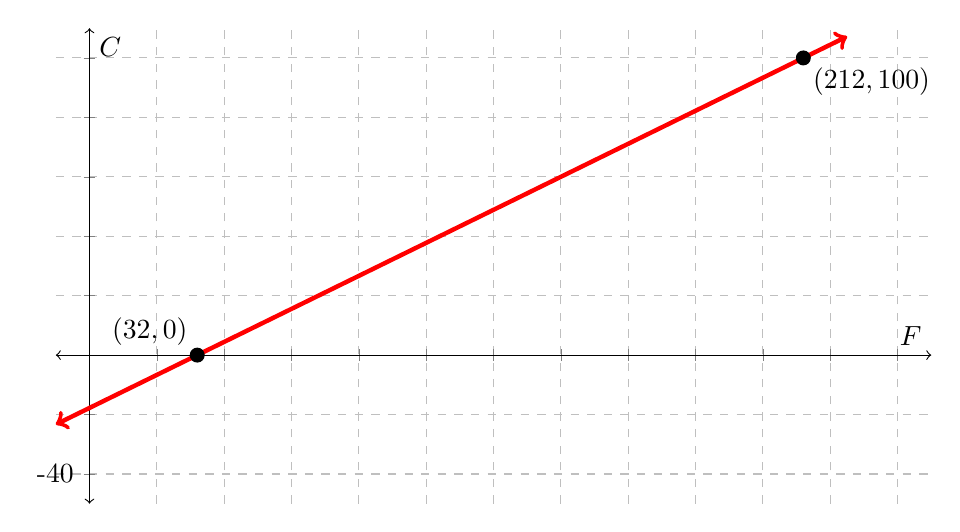
\begin{tikzpicture}
            \begin{axis}[
                %    axis y line = left,
                %    axis x line = bottom,
                    xlabel={$F$},
                    xtick       = {-40,-20,20,40,60,80,100,120,140,160,180,200,220,240},
                    xticklabels = {-40},
                    ylabel={$C$},
                    ytick       = {-40,-20,20,40,60,80,100},
                    yticklabels = {-40},
                    samples     = 160,
                    %domain      = -1:5,
                    %restrict y to domain=-1:5,
                    xmin = -10, xmax = 250,
                    ymin = -50, ymax = 110,
                    grid=both, grid style=dashed,
                    width=5in, height=3in
                  ]
                  \draw[ultra thick,red,<->] (-10,-23.33333) -- (225,107.22222222);
                  %\filldraw (-40,-40) circle (2.5pt);
                  \filldraw (32,0) circle (2.5pt) node[anchor=south east]{$(32,0)$};
                  \filldraw (212,100) circle (2.5pt) node[anchor=north west]{$(212,100)$};
            \end{axis}
        \end{tikzpicture}
\end{center}

    \begin{itemize}
    
    \item[(a)] What is the {\bf net change} of the temperature in degrees Fahrenheit as the temperature in degrees Celsius changes from water's freezing point to water's boiling point?
    
    \item[(b)] What is the {\bf average rate of change} of the temperature in degrees Fahrenheit as the temperature in degrees Celsius changes from water's freezing point to water's boiling point? What are the {\bf units} of measurement of this average rate of change?
    
    \item[(c)] What is the {\bf slope} of the graph depicted above? What is the {\bf equation} of the graph depicted above?
    
    \item[(d)] Write a sentence describing what the slope of the graph represents in this context.\\ 
    ({\bf Note:} ``in this context" means your answer must clearly relate to the scenario described in the problem - a graph relating temperature $C$ in degrees Celsius to temperature $F$ in degrees Fahrenheit. Answers like ``rise over run" are not in-context.)

    \item[(e)] ({\bf Challenge!}) At both the freezing point and boiling point of water, the temperatures in degrees Fahrenheit are numerically greater than the corresponding temperatures in degrees Celsius. Are there any examples of temperatures in degrees Fahrenheit that are numerically {\bf less than} the corresponding temperatures in degrees Celsius? Is there an example of a temperature in degrees Fahrenheit that are numerically {\bf equal} to the corresponding temperature in degrees Celsius? Explain.
    
    \end{itemize}

\item 

\end{enumerate}

\section{Exercise B Extra Extra Practice}

\begin{enumerate}\setcounter{enumi}{2}

\item The graph below depicts the relationship between ounces and pounds with two points plotted.

\begin{center}
        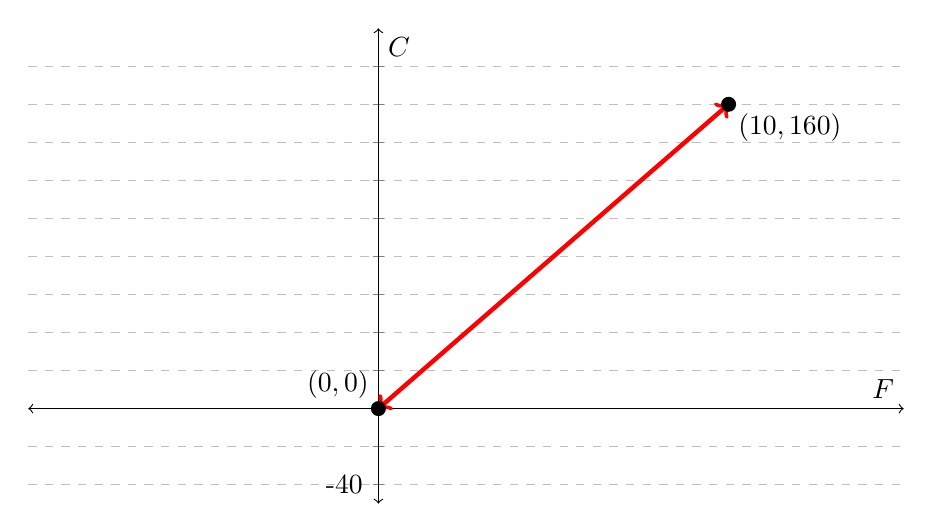
\begin{tikzpicture}
            \begin{axis}[
                %    axis y line = left,
                %    axis x line = bottom,
                    xlabel={$F$},
                    xtick       = {-40,-20,20,40,60,80,100,120,140,160,180,200,220,240},
                    xticklabels = {-40},
                    ylabel={$C$},
                    ytick       = {-40,-20,20,40,60,80,100, 120, 140, 160, 180},
                    yticklabels = {-40},
                    samples     = 160,
                    %domain      = -1:5,
                    %restrict y to domain=-1:5,
                    xmin = -10, xmax = 15,
                    ymin = -50, ymax = 200,
                    grid=both, grid style=dashed,
                    width=5in, height=3in
                  ]
                  \draw[ultra thick,red,<->] (0,0) -- (10,160);
                  %\filldraw (-40,-40) circle (2.5pt);
                  \filldraw (0,0) circle (2.5pt) node[anchor=south east]{$(0,0)$};
                  \filldraw (10,160) circle (2.5pt) node[anchor=north west]{$(10,160)$};
            \end{axis}
        \end{tikzpicture}
\end{center}

    \begin{itemize}
    
    \item[(a)] What is the {\bf net change} of the in ounces with respect to pounds between the marked points?
    
    \item[(b)] What is the {\bf average rate of change}? What are the {\bf units} of measurement of this average rate of change? 
    
    \item[(c)] What is the {\bf slope} of the graph depicted above? What is the {\bf equation} of the graph depicted above?
    
    \item[(d)] Write a sentence describing what the slope of the graph represents in this context.\\ 
    ({\bf Note:} ``in this context" means your answer must clearly relate to the scenario described in the problem.
    \end{itemize}

\item 

\end{enumerate}
\end{document}